\documentclass[../main.tex]{subfiles}

\begin{document}

\section*{第1問}

{\bf [解]}
$P(1+2t,\, t,\, -2-t)$，$Q(1+s,\, 2-s,\, -3+s)$，$R(1+u,\, -1+2u,\, u)$とおく．

$Q$，$R$が垂足だから，$\overrightarrow{PQ}\perp m$，$\overrightarrow{PR}\perp n$となる．

\begin{align*}
\begin{pmatrix} s-2t \\ 2-s-t \\ -1+s+t \end{pmatrix}\cdot\begin{pmatrix}1\\-1\\1\end{pmatrix}=0
&\iff (s-2t)-(2-s-t)+(-1+s+t)=0\\
&\iff 3s-3=0 \iff s=1，\\[4pt]
\begin{pmatrix} u-2t \\ -1+2u-t \\ 2+u+t \end{pmatrix}\cdot\begin{pmatrix}1\\2\\1\end{pmatrix}=0
&\iff (u-2t)+2(-1+2u-t)+(2+u+t)=0\\
&\iff 6u-3t=0 \iff u=\frac{1}{2}t
\end{align*}

だから，$(s,u)=\left(1,\dfrac{1}{2}t\right)$である．

\begin{align*}
\overline{PQ}^2&=(s-2t)^2+(s+(t-2))^2+(s+(t-1))^2\\
&=3s^2-6s+6t^2-6t+5\\
&=6t^2-6t+2\quad(s=1\text{を代入})，\\[4pt]
\overline{PR}^2&=(u-2t)^2+(2u-(t+1))^2+(u+(t+2))^2\\
&=6u^2-6tu+6t^2+6t+5\\
&=\frac{9}{2}t^2+6t+5\quad\left(u=\frac{1}{2}t\text{を代入}\right)．
\end{align*}

だから，$f(t)=\overline{PQ}^2+\overline{PR}^2$とすると
\begin{align*}
f(t)=\frac{21}{2}t^2+7．
\end{align*}

これは$t=0$で最小値$7$をとる．この時$P(1,0,-2)$である．

\newpage

\section*{第2問}

{\bf [解]}
$n$秒後に異なる点にいる確率を$Q(n)$とし，同じ点にいる確率を$P(n)$とする．

$2$つの粒子が同じ点にいる状態からは，各粒子が独立に残り$2$頂点のいずれかへ等確率で移動するので，
次に同じ点にいる確率は$\dfrac12\cdot\dfrac12+\dfrac12\cdot\dfrac12=\dfrac12$である．

$2$つの粒子が異なる点にいる状態からは，同様に考えて，次に同じ点にいる確率は$\dfrac12\cdot\dfrac12=\dfrac14$である．

上図から
\begin{align*}
P(n+1)&=\frac12P(n)+\frac14Q(n)\\
&=\frac12P(n)+\frac14(1-P(n))\\
&=\frac14P(n)+\frac14
\end{align*}

$P(1)=\dfrac12$だから，くり返し用いて，
\begin{align*}
P(n)&=\left(\frac14\right)^{n-1}\left(\frac12-\frac13\right)+\frac13\\
&=\frac13\left\{1+\frac12\left(\frac14\right)^{n-1}\right\}．
\end{align*}

したがって，$p(n)=\dfrac13\left\{1+\dfrac12\left(\dfrac14\right)^{n-1}\right\}$である．

\newpage

\section*{第3問}

{\bf [解]}
$\angle A=\theta$とおく．内角の正条件から
\begin{align*}
0<\theta，\ 0<2\theta，\ 0<\pi-3\theta \iff 0<\theta<\frac{\pi}{3}\quad\cdots①
\end{align*}
である．

\begin{figure}[htb]
\centering
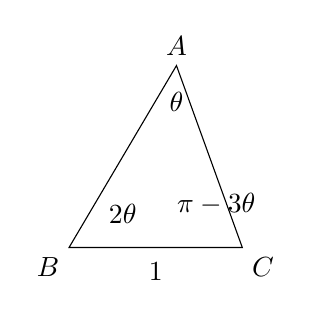
\begin{tikzpicture}[scale=2.2]
  \coordinate (B) at (0,0);
  \coordinate (C) at (1,0);
  \coordinate (A) at (0.62,1.05);
  \draw (A) -- (B) -- (C) -- cycle;
  \node[above] at (A) {$A$};
  \node[below left] at (B) {$B$};
  \node[below right] at (C) {$C$};
  \node[below=2pt] at (0.5,0) {$1$};
  \node[above=2pt] at (0.31,0.05) {$2\theta$};
  \node[above=2pt] at (0.85,0.1) {$\pi-3\theta$};
  \node[below=6pt] at (A) {$\theta$};
\end{tikzpicture}
\caption{$\triangle ABC$と角$\theta$，$2\theta$，$\pi-3\theta$の関係}
\end{figure}

正弦定理より
\begin{align*}
\frac{\overline{AB}}{\sin(\pi-3\theta)}=\frac{1}{\sin\theta}
\quad\therefore\ \overline{AB}=\frac{\sin3\theta}{\sin\theta}=3-4\sin^2\theta\quad\cdots②
\end{align*}

以下，$c=\cos\theta$，$s=\sin\theta$とする．$\triangle ABC$の面積$T$は②から
\begin{align*}
T&=\frac12\overline{AB}\cdot\overline{BC}\cdot\sin2\theta\\
&=\frac12(3-4s^2)\cdot2sc\\
&=(3-4s^2)sc
\end{align*}

これを$\theta$で微分して，
\begin{align*}
T'&=3\cos2\theta-4(3s^2c^2+(-s)\cdot s^3)\\
&=3(1-2s^2)-4s^2(3c^2-s^2)\\
&=3(1-2s^2)-4s^2(3-4s^2)\\
&=16t^2-18t+3\quad(t=s^2)
\end{align*}

$16t^2-18t+3=0$を解くと$t=\dfrac{9\pm\sqrt{33}}{16}$であり，①の範囲（$0<t<3/4$）に入るのは$t=\dfrac{9-\sqrt{33}}{16}$のみだから，下表を得る．

\begin{center}
\begin{tabular}{c|ccccc}
$\theta$ & $0$ & & & & $\pi/3$ \\
\hline
$t$ & $0$ & & $\dfrac{9-\sqrt{33}}{16}$ & & $3/4$ \\
\hline
$T'$ & & $+$ & $0$ & $-$ & \\
\hline
$T$ & & $\nearrow$ & （極大） & $\searrow$ & \\
\end{tabular}
\end{center}

したがって，もとめるのは
\begin{align*}
\cos\angle B=\cos2\theta=1-2t=1-\frac{9-\sqrt{33}}{8}=\frac{-1+\sqrt{33}}{8}．
\end{align*}

\newpage

\section*{第4問}

{\bf [解]}
$f(x)=\dfrac{ax+b}{x^2+x+1}$とする．$y=f(x)$とおけば，与式は
\begin{align*}
y^3-2y^2-y+2\ge0
\end{align*}
すなわち
\begin{align*}
(y-1)(y^2-y-2)\ge0 \iff (y-1)(y-2)(y+1)\ge0
\end{align*}
\begin{align*}
\therefore\ -1\le y\le1\ \text{または}\ 2\le y\quad\cdots①
\end{align*}

したがって，全ての$x$で①が成立すれば良い．$f(x)\xrightarrow{x\to\pm\infty}0$かつ，$x^2+x+1>0$から$f$が連続であることより，$2\le y$となる$x$がある時，①が全ての$x$で成立することはなく適さない．

よって，$-1\le y\le1$のみ調べる．
\begin{align*}
-(x^2+x+1)\le ax+b\le x^2+x+1
\end{align*}
\begin{align*}
-x^2-(a+1)x-1\le b\le x^2+(1-a)x+1\quad\cdots②
\end{align*}

②の右辺の最小値は$x=\dfrac{a-1}{2}$の時の$1-\left(\dfrac{1-a}{2}\right)^2=\dfrac{-a^2+2a+3}{4}$，
左辺の最大値は$x=-\dfrac{a+1}{2}$の時の$\dfrac{(a+1)^2}{4}-1=\dfrac{a^2+2a-3}{4}$だから，全ての$x$で②が成立する条件は，
\begin{align*}
\frac{a^2+2a-3}{4}\le b\le\frac{-a^2+2a+3}{4}．
\end{align*}

これを図示して，以下斜線部（境界含む）．

\begin{figure}[htb]
\centering
\begin{tikzpicture}[scale=1.15, >=stealth]
  \begin{axis}[
      axis lines=middle,
      xlabel={$a$}, ylabel={$b$},
      xmin=-2.3, xmax=2.3, ymin=-1.6, ymax=1.6,
      xtick={-1.7320508,1.7320508}, xticklabels={$-\sqrt3$,$\sqrt3$},
      ytick=\empty,
      clip=false,
      domain=-1.7320508:1.7320508, samples=100, smooth,
    ]
    \addplot[name path=upper, thick] {(-x^2+2*x+3)/4};
    \addplot[name path=lower, thick] {(x^2+2*x-3)/4};
    \addplot[gray!25] fill between[of=upper and lower];
  \end{axis}
\end{tikzpicture}
\caption{条件②を満たす$(a,b)$の範囲（斜線部）}
\end{figure}

\newpage

\section*{第5問}

{\bf [解]}
$a^3+b^3=(a+b)(a^2-ab+b^2)$である．以下合同式の法を$3$とする．対称性から，$(a,b)\equiv(1,1),(1,2),(2,2)$の時をしらべれば良い．

\begin{itemize}
\item[$\circ$] $(a,b)\equiv(1,1)$の時，$a^3+b^3\equiv2$となり不適．
\item[$\circ$] $(a,b)\equiv(2,2)$の時，$a^3+b^3\equiv16\equiv1$，同様に不適．
\end{itemize}

だから，$(a,b)\equiv(1,2)$が必要である．この時，$a+b\equiv0$，$a^2-ab+b^2\equiv0$から，$a^3+b^3$は少なくとも$9$で割り切れる．そこで，$m,n\in\mathbb{Z}_{\ge0}$として，
\begin{align*}
a=3m+1，\quad b=3n+2\quad\cdots①
\end{align*}
とおく．
\begin{align*}
a+b&=3(m+n+1)，\\
a^2-ab+b^2&=(9m^2+6m+1)+(9n^2+12n+4)-(9mn+3n+6m+2)\\
&=9m^2+9n^2-9mn+9n+3
\end{align*}

から，$a^2-ab+b^2$は$9$で割り切れず，$a+b$が$81$で割り切れるには$a+b$が$27$で割り切れなければならない．そこで，$\ell\in\mathbb{N}$として
\begin{align*}
a+b=27\ell\quad\cdots②
\end{align*}
とする．それが条件．$A=a^2+b^2$として，
\begin{align*}
A&=\frac12\left\{(a+b)^2+(a-b)^2\right\}\\
&=\frac12\left\{(27\ell)^2+(27\ell-2b)^2\right\}
\end{align*}

$\ell=1$の時，これは$b=14(\equiv2)$で最小値$365$をとる．この時$a=13$である．一方，$\ell\ge2$の時
\begin{align*}
A\ge\frac12(27\ell)^2\ge\frac12\cdot4\cdot27^2=729\cdot2>365
\end{align*}
から，$A$が$365$より小さくなることはない．以上から，$(a,b)=(13,14)$で$\min(a^2+b^2)=365$．この時対称性から$(a,b)=(14,13)$も解である．

\bigskip
\noindent{\bf [解2]}
$(a+b)^3=a^3+b^3+3ab(a+b)$から，$a^3+b^3\equiv0\pmod{81}$の時，$a+b$が$3$で割り切れ
\begin{align*}
a+b=3c
\end{align*}
とおける．代入・整理して
\begin{align*}
9abc=27c^3-(a^3+b^3)
\end{align*}
だから，$a,b\not\equiv0\pmod3$から，$c\equiv0\pmod3$である．この時
\begin{align*}
a^3+b^3=27c^3-9abc
\end{align*}
より，$a^3+b^3$は$81$で割り切れる．よって，条件は，$\ell\in\mathbb{N}$として
\begin{align*}
\ulcorner\, a,b\not\equiv0\pmod3\text{かつ}a+b=27\ell\,\urcorner
\end{align*}
（以下省略）

\bigskip
\noindent{\bf [注]}
最後の$a+b=27\ell$以下，図示してみると$\ell=1$で$\min$なのは明らかで，$\ell\ge2$の時
\begin{align*}
a^2+b^2\ge(27)^2+(27)^2>365
\end{align*}
を得る．

\newpage

\section*{第6問}

{\bf [解]}
$C_2:x^2+y^2=r^2\ (x,y>0)$とする．まず$C_1$，$C_2$が2点で交わる条件から
\begin{align*}
\sqrt2<r\quad\cdots①
\end{align*}
である．2交点$A(r\cos\alpha,r\sin\alpha)$，$B(r\cos\beta,r\sin\beta)$（$0<\alpha<\beta<\pi/2$）とおくと，対称性から
\begin{align*}
\beta=\frac\pi2-\alpha\quad\cdots②
\end{align*}
となる．次に，$C_1$が$A$を通る条件から
\begin{align*}
r\sin\alpha=\frac{1}{r\cos\alpha}\quad\cdots③
\end{align*}

$A$における接線$\ell$の傾きは$-\dfrac{1}{r^2\cos^2\alpha}$である．$\angle OAC=\pi/6$（$C$は$\ell$と$x$軸の交点）という条件のもとで角の関係を整理し，$\tan\alpha=t$とおくと
\begin{align*}
\frac{\sqrt3}{3}=\frac{t+r^2t+1}{r^2-t^2-t}\quad\cdots④
\end{align*}
を得る．ここで，③の両辺に$\dfrac{1}{\cos\alpha}$をかけて整理すると
\begin{align*}
r^2t=t^2+1\quad\cdots⑤
\end{align*}

④，⑤から
\begin{align*}
r^2-t^2-t&=\sqrt3(t^2+r^2t+1)\\
t^3+\sqrt3t^2+(\sqrt3r^2+1)t+\sqrt3-r^2&=0\\
(t+\sqrt3)(r^2t-1)+(\sqrt3r^2+1)t+\sqrt3-r^2&=0\\
r^2(r^2t-1)+(\sqrt3r^2-1)t+(\sqrt3r^2+1)t-r^2&=0\\
(r^4+2\sqrt3r^2)t&=2r^2
\end{align*}
であり，
\begin{align*}
t=\frac{2}{r^2+2\sqrt3}
\end{align*}

であり，⑤を代入して，
\begin{align*}
t^2+2\sqrt3t-1=0
\end{align*}
\begin{align*}
t=-\sqrt3\pm2
\end{align*}

$t>0$から複号正を採用して，
\begin{align*}
t=2-\sqrt3=\tan15^\circ，\quad r=2\quad（①を満たす）\quad\cdots\text{＊}
\end{align*}

だから，$0<\alpha<\pi/4$から$\alpha=15^\circ$，⑥である．題意の面積$S$として
\begin{align*}
S=(\text{扇形}OAB\text{の面積})-(\text{$C_1$と線分}AB\text{に囲まれた部分の面積})\quad\cdots⑦
\end{align*}
であり，
\begin{align*}
\text{扇形}OAB&=\frac12r^2\left(\frac\pi2-\frac\pi6\right)=\frac23\pi，\\
\text{$C_1$と線分}AB\text{に囲まれた部分}&=\int_{\sin\alpha}^{\cos\alpha}\frac{1}{x}\,dx=\log\frac1t
\end{align*}

を代入して，＊，⑦から
\begin{align*}
S=\frac23\pi-\log\frac{1}{2-\sqrt3}=\frac23\pi-\log(2+\sqrt3)．
\end{align*}

\bigskip
\noindent{\bf [解2]}
対称性から，$y=x$の方を$\ell$とする．$A\left(p,\dfrac1p\right)$とする（$0<p<1$）．$A$での接線の傾きは$-\dfrac{1}{p^2}$であり，$\ell$と$x$軸の交点を$C$として，$\overline{OA}=\overline{AC}$となる．（$\because$ $OA$の傾き符号）$\angle AOC>\pi/4$から題意の条件は$\angle OAC=\pi/6$である．この時$\angle AOC=\dfrac{5}{12}\pi$となる．
\begin{align*}
\tan\frac{5}{12}\pi=2+\sqrt3
\end{align*}
だから，
\begin{align*}
\frac{1}{p^2}=\tan\frac{5}{12}\pi=2+\sqrt3\quad\therefore\ p=\sqrt{2-\sqrt3}
\end{align*}

以下，$\alpha=\sqrt{2-\sqrt3}$，$\beta=\sqrt{2+\sqrt3}$とする．
\begin{align*}
S&=\text{（扇形）}-\text{（$C_1$に囲まれた部分）}\\
&=\frac12(\alpha^2+\beta^2)\cdot\frac\pi3-\int_\alpha^\beta\frac1x\,dx\\
&=\frac23\pi-\log(2+\sqrt3)．
\end{align*}

\newpage

\end{document}
